\chapter{Insiemi ricorsivi e ricorsivamente enumerabili}

% CHIARA

\section{Definizioni}

\begin{defi}
Un insieme $A$ di numeri naturali \`e \underline{ricorsivo} se e solo se esiste una
funzione ricorsiva totale $f$ tale che $\forall x,\ x\in A\rightarrow f(x)=1\mbox{\ e\ }x\in\bar{A}\rightarrow f(x)=0$.
\end{defi}

Intuitivamente, $A$ \`e ricorsivo se esiste una procedura effettiva
per decidere, qualunque sia l'$x$ dato, se $x\in A$ o $x\in\bar{A}$.
Dal capitolo precedente ricordiamo che avere "`una procedura effettiva"' equivale ad avere "`una funzione ricorsiva primitiva totale"'.

\begin{defi}Si dice \underline{funzione caratteristica} di un insieme ricorsivo $A$ una funzione $c_A$ tale che\\

$c_A(x)=\left\{ \begin{array}{cc}
1 & se\ x\in A\\
0 & se\ x\notin A\end{array}\right.$
\end{defi}

\`E immediato che un insieme possiede una funzione caratteristica se e solo se \`e ricorsivo.\\
Esempi:
\begin{enumerate}
\item Numeri pari;
\item $\mathbb{N}$ e $\emptyset$;
\item Qualsiasi insieme finito;
\item Qualunque complemento di un insieme finito.
\end{enumerate}
Infatti per ognuno di questi insiemi \`e facile scrivere una funzione caratteristica.

\begin{defi}
(Post[1922], Kleene[1936]) Un insieme di numeri naturali $A$ si dice
\underline{ricorsivamente enumerabile} (abbreviato \underline{r.e.}) se esiste
una funzione ricorsiva parziale il cui dominio \`e esattamente $A$
(o equivalentemente, esiste una funzione ricorsiva parziale che \`e definita
solo per gli input appartenti ad $A$, cio\`e se tale funzione converge, cio\`e termina, se e solo se gli input dati appartengono ad $A$)
\end{defi}

Possiamo introdurre la definizione di una funzione che caratterizza gli insiemi r.e. (similmente a quanto fatto gi\`a fatto con gli insiemi ricorsivi).

\begin{defi}
Si definisce \underline{funzione semicaratteristica} di un insieme r.e. $A$ una funzione ricorsiva
parziale $sc_A$ tale che\\

$sc_A$ converge se e solo se $x \in A$

e $sc_A(x)=1$ dove converge.\footnote{Questa definizione classicamente equivale a 
$sc_A(x)=\left\{ \begin{array}{cc}
1 & se\ x\in A\\
non\ definita & se\ x\notin A\end{array}\right.$
Ma intuizionisticamente questa seconda non \`e del tutto corretta perch\`e presuppone che si sia in grado di decidere se un elemento appartiene o non appartiene ad $A$. Con la definizione data, invece, basta saper decidere se un elemento appartiene ad $A$ e la funzione risulta automaticamente non definita per tutti i valori che non stanno in $A$}

\end{defi}

Un insieme \`e r.e. se e solo se possiede una funzione semicaratteristica. Infatti una funzione come quella della definizione di r.e. (cio\`e definita solo sugli input appartenenti ad A) pu\`o sempre essere ricondotta ad una funzione semicaratteristica (cio\`e definita solo sugli input appartenenti ad A e che per questi restituisca uno).

Un esempio di insieme r.e. potrebbe essere il seguente:

$A=\{y$ t.c. $y$ \`e uno degli output della funzione $f\}$ per una qualche funzione $f$ fissata.

Consideriamo la funzione $g(y)$ che, dato un $y$, mi restituisce il valore $x$ tale che $f(x)=y$. 

Se $y$ \`e un output della funzione, calcolandola in tutto il suo dominio, prima o poi trover\`o un qualche valore $x$ che dato come input alla funzione $f$ mi restituisce $y$. Dunque $g(y)$ termina e ha come output $x$.

Se $x$ non \`e un output della funzione, pur calcolandola in tutto il dominio, non trover\`o mai un valore che dato in input alla funzione mi restituisca $x$. Dunque il mio procedimento non termina mai e $g(y)$ non \`e definita.

Adesso possiamo vedere chiaramente che:

\begin{thm}
\label{thm:1}
Ogni insieme ricorsivo \`e anche r.e.

\end{thm}

\begin{proof}

$A$ \`e un insieme ricorsivo. Allora, per definizione di ricorsivo, esiste una funzione $f$ tale che

$f(x)=1$ se $x \in A$

$f(x)=0$ se $ x \notin A$

Definiamo la seguente funzione: $g(x)=s(z(\mu y.(f(x)-1)))$.

se $x \in A$ allora $f(x)=1$, dunque la minimizzazione interna a $g(x)$ termina e $g(x)$ restituisce il valore $1$.

se $x \notin A$ allora $f(x)=0$, dunque la minimizzazione interna a $g(x)$ non termina mai e $g(x)$ non risulta definita.

Si vede che $g(x)$ \`e una funzione ricorsiva parziale con dominio $A$, in particolare si tratta della sua funzione caratteristica. Dunque $A$ \`e un insieme r.e.

\end{proof}

\section{Caratterizzazione insiemi ricorsivi ed r.e.}

\begin{thm}
\label{thm:3}
Sia $A$ un insieme abitato e infinito. Allora sono equivalenti:

\begin{itemize}
\item [1)] $A$ \`e un insieme ricorsivo 

\item [2)] $A$ \`e immagine di una funzione $f$ non decrescente ricorsiva.
\end{itemize}

\end{thm}

\begin{proof}
$1) \Rightarrow 2)$ Poich\`e $A$ \`e abitato, siamo in grado di trovare il suo elemento minimo, che chiamiamo $a$. Definiamo la seguente funzione:

$$f(0)=a$$

$f(n+1)=\left\{ \begin{array}{cc}
n+1 & se\ n+1\in A\\
f(n) & se\ n+1\notin A\end{array}\right.$

Si vede facilmente che la funzione $f$ \`e non decrescente. Per vedere che $f$ \`e ricorsiva, possiamo scriverla in questo modo, usando la ricorsione e la funzione caratteristica di $A$.


$\left\{ \begin{array}{l}
h(\bar{x},0)=a\\
h(\bar{x},s(y))=s(y)c_A(s(y))+h(\bar{x},y)(1-c_A(s(y)))\end{array}\right.$

Inoltre si vede facilmente che $f$ stampa tutti e soli gli elementi di $A$. Dunque abbiamo trovato la funzione che cercavamo.
\bigskip

$2) \Rightarrow 1)$ $A$ \`e immagine di una funzione $f$ ricorsiva non decrescente. Dato un elemento $z$, voglio capire se questo appartiene o meno ad $A$. 

Poich\`e $A$ \`e infinito, esister\`a sicuramente un suo elemento che sia pi\`u grande di $z$. Poich\`e $A$ \`e immagine di $f$, tale elemento potr\`a essere scritto come immagine di un qualche $x$. Prendiamo allora il minimo $x$ tale che $f(x)>z$. Se $z$ appartiene ad $A$, deve esistere un qualche $y$ tale che $f(y)=z$. Questo $y$ non pu\`o chiaramente essere pi\`u grande di $x$, perch\`e $f(x)>z$ e $f$ \`e non decrescente, quindi qualunque elemento pi\`u grande di $x$ ha immagine pi\`u grande di $z$. Dunque per verificare se $z$ appartiene ad $A$, mi basta controllare se appartiene a $\{f(0),...,f(x)\}$, che \`e un insieme finito. 

$$z \in A \Longleftrightarrow z \in \{f(0),...,f(x)\}$$

Poich\`e la $x$ cercata esiste \`e possibile trovarla con un numero finito di passaggi, e poich\`e per capire se $z$ \`e immagine di $f$ mi basta controllare all'interno di un insieme finito allora ho una procedura che termina sicuramente e che sa dirmi se $z$ appartiene o meno ad $A$. Dunque A \`e un insieme ricorsivo.

\end{proof}

Dunque un insieme ricorsivo pu\`o essere sempre listato con una funzione ricorsiva non decrescente. 

\begin{thm}
Gli insiemi r.e. sono chiusi per intersezione finita e per unione finita.
\end{thm}
 
\begin{proof}
Dimostriamo la chiusura per l'unione. Siano $A_{1}$, $A_{2}$, $A_{3}$, ecc gli insiemi r.e. di cui $A_{U}$ \`e l'unione. Ognuno di questi insiemi ha una funzione semicaratteristica associata. La funzione semicaratteristica dell'insieme unione pu\`o essere calcolata informalmente in questo modo. Sia $a$ l'elemento che vogliamo stabilire se appartiene ad $A_{U}$. Calcoliamo contemporaneamente le funzioni semicaratteristiche dei vari insiemi originali. Eseguiamo cio\`e un passo della prima macchina di Turing, poi un passo della seconda e cos\`i via. Quando tutte le macchine hanno eseguito un passo calcoliamo il secondo passo di ogni funzione. Se una delle funzioni semicaratteristiche degli insiemi originari termina, fermiamo la computazione e restituiamo 1. Altrimenti continuamo con la computazione (la computazione diverge). La funzione semicaratteristica appena descritta \`e ricorsiva parziale e restituisce 1 se $a\in A_{U}$.
Dimostriamo la chiusura per l'intersezione. Definiamo una funzione semicaratteristica in maniera del tutto simile a quella utilizzata per l'unione. Questa volta, per di pi\`u, possiamo eseguire le varie funzioni semicaratteristiche in maniera seriale, cio\`e una dopo l'altra. Quando tutte hanno terminato, restituiamo 1. Altrimenti continuiamo la computazione (divergendo).
\end{proof}

\begin{thm}
Se $\psi$ \`e una funzione ricorsiva parziale e $A$ \`e ricorsivamente
enumerabile, allora $\psi^{-1}(A)$ \`e ricorsivamente enumerabile.
\end{thm}

\begin{proof}

$A$ \`e un insieme r.e., dunque, per definizione di r.e., esiste una funzione ricorsiva parziale $f$ di cui $A$ \`e dominio. Consideriamo ora la funzione $f \circ \psi$. Poich\`e $f$ \`e definita solo per input appartenenti ad $A$, la funzione $f \circ \psi$ \`e definita solo per quegli elementi che hanno immagine, rispetto alla funzione $\psi$, che appartiene ad $A$, e cio\`e per gli elementi di $\psi^{-1}(A)$. Dunque $\psi^{-1}(A)$ \`e dominio della funzione $f \circ \psi$, che \`e una funzione ricorsiva, in quanto composizione di due funzioni ricorsive. Dunque $\psi^{-1}(A)$ \`e un insieme r.e.  

\end{proof}

\section{Coda di rondine e codifica di coppia}

Vediamo ora di affrontare il problema di scorrere tutte le possibili coppie di numeri naturali. Se mi limito ad incrementare uno dei termini della coppia,(ad esempio prendendo in ordine le coppie (0,0),(0,1),(0,2),(0,3),...) non arriver\`o mai a considerare tutte le coppie possibili, perch\`e l'altro termine della coppia resta sempre fisso sullo stesso valore. Bisogna trovare un metodo alternativo. Una soluzione \`e data dalla Coda di Rondine.

Si tratta praticamente di procedere, come in figura, a zig zag lungo una tabella, che ha fissato in ogni riga il valore del primo elemento della coppia, e in ogni colonna il valore del secondo. Risulta evidente dall'immagine che in questo modo vengono considerate tutte le possibili coppie di numeri.

\begin{figure}
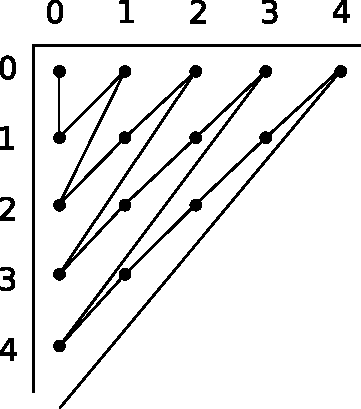
\includegraphics{img/dovetail.pdf}
\end{figure}

Un altro strumento che viene utilizzato \`e la codifica di coppia. Tale strumento viene utilizzato molto spesso in calcolabilit\`a, ed \`e alla base (una volta generalizzato per un numero arbitrario di argomenti) del meccanismo per cui possiamo sempre approssimare una funzione con $N$ argomenti con una funzione ad $n$ argomenti con $N>n$. Praticamente questa ci permette di associare ad ogni possibile coppia un numero naturale e viceversa, in questo modo:

\begin{equation}\left\langle x,y \right\rangle = 2^x(2y+1)-1.\end{equation}

La funzione di codifica \`e reversibile, cio\`e dato il numero che codifica la coppia possiamo calcolare i due numeri che la formano:

\begin{equation}\pi_{1}(z) = \mu x((z+1)/2^x\ sia \ dispari)\end{equation}
\begin{equation}\pi_{2}(z) = ((z+1)/2^{\pi_{1}(z)} -1)/2 \end{equation} 

Questo metodo sar\`a pi\`u utilizzato della coda di rondine, in quanto, oltre a darci un ordine con cui scorrere tutte le coppie, ci permette di associarle ad un numero e di passare in modo molto veloce da numero a coppia e da coppia a numero. Inoltre, la codifica di coppia pu\`o essere utilizzata per codificare triplette o n-uple di numeri. Per le triplette basta, ad esempio, codificare come coppia gli ultimi due elementi, ottenendo cos\`i una coppia, e poi codificare questa di nuovo.

% ALESSANDRO

\section{Predicati e insiemi}

%%%%%%%%%%%%%%%%%%%%%%%%%%%%%%%%%%%%%%%%%%%%%%%
%
% PREDICATI E INSIEMI
%
%%%%%%%%%%%%%%%%%%%%%%%%%%%%%%%%%%%%%%%%%%%%%%%

Data la necessit\`{a} di introdurre il concetto di \textit{predicato}, \`{e} importante notare che:
\begin{itemize}
 \item un predicato si dice \textit{decidibile} quando si \`{e} costruttivamente in grado di determinare se esso vale o non vale su di un argomento
 \item un predicato si dice \textit{semidecidibile} quando si \`{e} costruttivamente in grado di determinare solo se se esso vale su di un argomento, mentre non si \`{e} in grado di farlo per quando non vale
\end{itemize}
Se si considerano le procedure effettive che caratterizzano se un predicato vale (o non vale) su di un argomento, \`{e} facile notare una diretta corrispondeza tra:
\begin{itemize}
 \item la procedura che caratterizza un predicato decidibile e la funzione caratteristica di un insieme ricorsivo
 \item la procedura che caratterizza un predicato semidecidibile e la funzione semicaratteristica di un insieme semidecidibile
\end{itemize}
in quanto gli elementi su cui il predicato vale formano un insieme che \`{e} il dominio della procedura che caratterizza il predicato stesso e, se la procedura è ricorsiva, e ovvio notare come tale insieme \`{e}:
\begin{itemize}
 \item \textit{ricorsivo} se il predicato \`{e} decidibile
 \item \textit{r.e.} se il predicato \`{e} semidecidibile
\end{itemize}
Nei teoremi che seguono quindi (e comunque in generale), i teoremi dimostrati per i predicati semidecidibili verranno assunti come validi anche per gli insiemi r.e..

%%%%%%%%%%%%%%%%%%%%%%%%%%%%%%%%%%
%
% N GODEL
%
%%%%%%%%%%%%%%%%%%%%%%%%%%%%%%%%%%

\section{Numero di G\"odel}

\begin{thm} Teorema di Forma Normale (Kleene [1936]):
Esiste una funzione primitiva ricorsiva $ U(x)$ e per ogni n $\ge1$ un predicato decidibile $T_{n} \left( e,\overrightarrow{x},z \right)$ tali che per ogni funzione ricorsiva $\varphi$ ad $n$ variabili esiste un numero $e$ per cui vale:
\begin{enumerate}
\item $\varphi^{\left( n \right)} \left( \overrightarrow{x}\right)\downarrow$ se e solo se $\exists z T_{n} \left(  e  , \overrightarrow{x}  , z \right)$  ;
\item $\varphi^{\left( n \right)}_{e} =  U \left( \mu  z   T_{n}\left( e,\overrightarrow{x},z\right) \right)   $ ;
\end{enumerate}
\end{thm}

$T_{n} \left( e,\overrightarrow{x},z \right)$ \`e chiamato "`Predicato T di Kleene"' e informalmente si legge: la macchina di Turing (o procedura equivalente per la \textit{Tesi di Church}) con indice $e$, applicata all'input $\overrightarrow{x}$ si ferma in $z_{1}$ passi con output $z_{2}$. L'argomento $z$ \`e la codifica della coppia $\langle  z_{1} , z_{2} \rangle$. Questo predicato \`e decidibile (ovvero la funzione che lo calcola \`e totale) dato che viene posto un limite rigido al numero di passi che la macchina deve eseguire cio\`{e} $z_1$.\\
In altri termini il predicato consiste di una procedura effettiva che esegue $z_1$ passi della e-esima macchina di Turing per poi andare a vedere se la macchina ha terminato, e se lo ha fatto, se ha ritornato il valore $z_1$, quindi sar\`{a} sempre in grado di dare una risposta, su ogni input $\Rightarrow$ \`{e} un predicato decidibile.\\
La codifica di coppia fa s\`i che vengano testati tutti i possibili valori di $z_1$ e $z_2$.\\
$U(x)$ \`{e} la funzione primitiva ricorsiva che prende la seconda componente della codifica di coppia dello $z$ per cui il predicato \textit{T di Kleene} vale.

\paragraph{\textbf{Un esempio molto informale}}

Per usare una metafora molto pittoresca, supponiamo di avere un appuntamento con la nostra ragazza (o ragazzo) al parco e che la funzione ricorsiva da calcolare sia "`la mia ragazza \`e arrivata"'. Se la nostra ragazza arriva puntuale \`e facile rispondere di s\`i immediatamente. Anche se il ritardo \`e breve, ad esempio 5 minuti, decidere se lei \`e arrivata \`e un compito abbastanza facile. Cosa succede per\`o se il ritardo si f\`a pi\`u consistente? L'unico modo per essere assolutamente certi che lei non arriver\`a, \`e di continuare ad aspettarla. Se per esempio dopo 2 settimane decidessimo arbitrariamente che lei non arriver\`a e lasciassimo il parco, lei potrebbe sempre arrivare con un ritardo di 2 settimane e 5 minuti. Per poi sentirci rinfacciare di esserci dimenticati! Allo stesso modo per\`o, continuare ad aspettare ci pone davanti allo spiacevole rischio di invecchiare all'infinito sulla panchina del parco in sua attesa. L'unica soluzione ragionevole \`e di decidere dopo un margine abbastanza largo se la nostra ragazza \`e venuta al nostro appuntamento oppure no.

Il predicato \textit{T di Kleene} \`e equivalente, per le funzioni ricorsive, a ci\`o che farebbe una persona normale in occasione di un appuntamento. Fissa un tempo limite (un determinato numero di passi nel nostro caso) per stabilire se per una determinata funzione ricorsiva con un determinato input si \`e avuta una convergenza su un determinato output.\\


Possiamo quindi considerare il numero $e$ come l'indice della funzione parziale ricorsiva per cui valgono (1) e (2) ed introdurre la nostra specifica notazione:
\begin{defi}
$
\varphi^{n}_{e} \left( o \left\lbrace e  \right\rbrace^n  \right)
$
\`e l' e-esima funzione parziale di n va\-ria\-bi\-li:
\[
\varphi^{\left( n \right)}_{e} \left( \overrightarrow{x}\right)\downarrow\ =\ U \left( \mu  z T_{n}\left(e,x_1,....,x_n,z \right) \right)
\]
\end{defi}
Il seguente teorema \`e una forma simmetrica del \textit{Teorema di Forma Normale di Kleene}:

\begin{thm}
Teorema di Enumumerazione: La sequenza $ \left\lbrace   \varphi^{n}_{e} \right\rbrace_{e \in w} $ \`e un elemento della enumerazione di funzioni parziali, nel senso che:

\begin{enumerate}
\item Per ogni e, $\varphi^{n}_{e}$ \`e una funzione parziale ricorsiva di $n$ variabili
\item Se $\psi$ \`e una funzione parziale ricorsiva di $n$ variabili, allora esiste un e tale che $\psi = \varphi^{n}_{e}$
\end{enumerate}
\end{thm}

\begin{proof}
Tutto segue dal Teorema di Forma Normale e dalla definizione di $\varphi^{n}_{e}$ :
$$\varphi \left( e,\overrightarrow{x} \right) = U \left( \mu  z   T_{n}\left( e,\overrightarrow{x},z\right) \right)$$
\end{proof}

L'indice di una funzione, conosciuto come numero di G\"odel, \`e un concetto molto importante che permette di identificare ogni possibile funzione ricorsiva (e quindi ogni possibile programma o macchina di Turing o procedura equivalente per la \textit{Tesi di Church}) e allo stesso tempo di riassumere ogni programma con un singolo numero. Questo \`e un concetto chiave della teoria della ricorsione, che aggiunge nuovo significato (oltre a quello immediato) ai numeri. Da questo momento in poi infatti, un numero non sar\`a pi\`u soltanto un input, un output o un pezzo di programma, ma un programma stesso. In ogni momento un programma potr\`a quindi fare riferimento ad un altro programma semplicemente "`chiamandolo per nome"' (cio\`e per il suo indice). Si potr\`{a} fornire come input a un programma un altro programma o restituire come output un programma. Cosa pi\`u incredibile, usando il suo indice un programma potr\`a riferirsi a se stesso durante la sua stessa computazione.

%%%%%%%%%%%%%%%%%%%%%%%%%%%%%%%%%%%%%%%%%%%%%%%
%
% PREDICATI
%
%%%%%%%%%%%%%%%%%%%%%%%%%%%%%%%%%%%%%%%%%%%%%%%

\section{Proprietà dei predicati semidecidibili}

\begin{thm}[Teorema di struttura]
$P(x)\subseteq\mathbb{N}^{k}$ predicato decidibile sse esiste $Q(x,z)\subseteq\mathbb{N}^{k+1}$ decidibile t.c. $P(x)=\exists z\ Q(x,z)$.
\end{thm}

\begin{proof}
($\Leftarrow$) sia $P(x)$ semidecidibile.\\
Possiamo quindi scrivere la sua funzione semicaratteristica
$$SC_{P}(x)\ converge\ a\ 1\ sse\ P(x)$$
che per definizione di insieme r.e. \`{e} una funzione ricorsiva.\\
Dato che ogni funzione ricorsiva \`{e} enumerabile esiste un $e\in\mathbb{N}$ per cui
$$SC_{P}(x)=\varphi_{e}(x)$$
Usando ora il predicato \textit{T di Kleene} possiamo scrivere
$$SC_{P}(x)=\exists z\ T(e,x,z)$$
Il predicato \textit{T di Kleene} \`{e} decidibile e, fissato $e$, possiamo scriverlo come $Q(x,z)$
$$SC_{P}(x)=\exists z\ Q(x,z)$$
Intuitivamente il teorema dice che nel cercare uno $z$ tale che $Q$ valga, partendo dal minimo $z$, se non lo si trova, si va avanti all'infinito.\\

($\Rightarrow$) sia $P(x)=\exists\ z Q(z,x)$ con $Q$ predicato decidibile.\\
Per dimostrare che $P(x)$ \`{e} semidecidible scriviamo la sua funzione semicaratteristica
$$SC_{P}(x)=s(z(\mu z.\ 1-\chi_{Q}(x,z)))$$
$SC_{P}$ \`{e} ricorsiva perch\'{e} definita per composizione di funzioni ricorsive ($\chi_{Q}$ \`{e} ricorsiva perch\'{e} $Q$ \`{e} decidibile) e minimalizzazione illimitata.
Quindi $P$ per la definizione di funzione semicaratteristica \`{e} semidecidibile.
\end{proof}
Questo teorema evidenzia come gli insiemi ricorsivi non siano chiusi rispetto all'esistenziale in quanto nel caso di un valore che non appartenga al dominio dell'insieme ricorsivo l'esistenziale divergerebbe.

\begin{thm}[Teorema di proiezione]
Sia $P(x,y) \subseteq\mathbb{N}^{k+1}$ predicato semidecidibile. Allora $S(x) = \exists x\ P(x,y)$ \`{e} semidecidibile.
\end{thm}

\begin{proof}
sia $P(x,y)$ semidecidibile.\\
Allora per il \textit{Teorema di struttura} esiste $Q(t,x,y)$ decidibile tale che:
$$P(x,y) = \exists t\ Q(t,x,y)$$
quindi possiamo riscrivere la conclusione del teorema come
$$S(x) = \exists x\ \exists t\ Q(t,x,y)$$
Usiamo ora la codifica di coppia per scorrere tutte le coppie $\langle x,t \rangle$ con un $w\subseteq\mathbb{N}$:
$$S(x) = \exists w\ Q(\pi_{2}(w),\pi_{1}(w),y)$$
che notiamo essere l'esistenziale di un predicato decidibile.
Per il \textit{Teorema di struttura} possiamo dunque concludere che $S(x)$ \`{e} semidecidibile.
\end{proof}
Anche questo teorema ci fornisce una nozione importante sugli insiemi, cio\`{e} che gli insiemi r.e. sono chiusi rispetto all'esistenziale, a differenza degli insiemi ricorsivi.

%%%%%%%%%%%%%%%%%%%%%%%%%%%%%%%%%%%%%%%%%%%%%%%
%
% CARATTERIZZAZIONI
%
%%%%%%%%%%%%%%%%%%%%%%%%%%%%%%%%%%%%%%%%%%%%%%%

\section{Caratterizzazione insiemi ricorsivi ed r.e. (continua)}

\begin{thm}
 \label{thm:2}
(Post[1943], Kleene[1943], Mostowski [1947]) Un insieme $A$ \`e ricorsivo se e solo se $A$ \`e r.e. e $A$ possiede un complementare $\bar{A}$ r.e..
\end{thm}

\begin{proof}

($\Rightarrow$) Assumendo che $A$ sia ricorsivo, per dimostrare che entrambi $A$ ed $\bar{A}$ sono r.e., definiamo le rispettive funzioni semicaratteristiche e le scriviamo come funzioni ricorsive:\\

$SC_{A}(x)\ converge\ a\ 1\ sse\ C_{A}(x) = 1 \Rightarrow SC_{A}(x) = s(z(\mu w.\ 1 - C_{A}(x)))$\\

$SC_{\bar{A}}(x)\ converge\ a\ 1\ sse\ C_{A}(x) = 0 \Rightarrow SC_{\bar{A}}(x) = s(z(\mu w.\ C_{A}(x)))$\\

Notiamo come l'utilizzo della minimalizzazione illimitata con parametro $w$ applicata ad un argomento inidipendente da $w$ stesso sia l'espediente che abbiamo per far divergere tutta la funzione nel caso non si verifichi proprio il valore che ci aspettiamo di $C_{A}(x)$.\\
Avendo definito due funzioni parziali ricorsive che hanno come dominio rispettivamente $A$ e $\bar{A}$, per la definizione di insieme r.e. possiamo concludere che $A$ e  $\bar{A}$ sono r.e..\\

($\Leftarrow$) Per dimostrare questa implicazione \`{e} necessario tenere presente che $A$ e $\bar{A}$ sono complementari per ipotesi, cio\`{e} che $A\cup\bar{A} = \mathbb{N}$.\\
Dati $A$ e $\bar{A}$ r.e., per le loro funzioni semicaratteristiche abbiamo che:
\begin{center}
$x\in{A}\Leftrightarrow SC_{A}(x)\ converge\ a\ 1$\\\end{center}
\begin{center}
$x\in{\bar{A}}\Leftrightarrow SC_{\bar{A}}(x)\ converge\ a\ 1$\\\end{center}

Ora, per il teorema di struttura dei predicati semidecibili esistono due predicati decidibili $R$ e $Q$ tali che:
\begin{center}
$x\in{A}\Leftrightarrow \exists y R(x,y)$\\\end{center}
\begin{center}
$x\in{\bar{A}}\Leftrightarrow \exists y Q(x,y).$\\\end{center}
con $y$ numero di passi.\\
Dalla premessa che $A\cup\bar{A} = \mathbb{N}$ vale che:\\
\[
\forall x \exists y (R(x,y) \vee Q(x,y))
\]
Definiamo ora la funzione
\[
f(x)=\mu y(R(x,y) \vee Q(x,y))
\]
\`{E} importante notare come solo uno ed esattamente uno tra $R(x,y)$ e $Q(x,y)$ possa valere su di un argomento.\\
$f$ \`{e} ricorsiva totale e ritorna il minimo numero di passi per cui, su un dato argomento $x$, o $R$ o $Q$ vale. Possiamo utilizzare sempre $f(x)$ come numero di passi per i predicati decibili dato che, per quanto visto sopra, solo uno dei due, con $f(x)$ passi varr\`{a}, caratterizzando l'appartennza o meno dell'argomento $x$ all'insieme $A$.\\
Scriviamo quindi la funzione che caratterizza $A$:

$$
c_{A}(x)=\begin{cases}
1\ se\ R(x,f(x))\cr
0\ se\ Q(x,f(x))\end{cases}
$$\\
che essendo una funzione definita per casi, \`{e} ricorsiva.\\
Per la definizione di insieme ricorsivo, concludiamo che $A$ \`{e} ricorsivo.
\end{proof} 

% ANDREA

\section{Un insieme r.e. non ricorsivo}

\begin{thm}
  Esiste un insieme ricorsivamente enumerabile ma non ricorsivo, chiamiamo tale insieme K.
\end{thm}

\begin{proof}
  Vediamo che è possibile definire una funzione di questo tipo:\\

  $\psi(x)=\left\{ \begin{array}{ll}
  1 & se\ \varphi_{x}(x)\ termina\\
  diverge & se\ \varphi_{x}(x)\ diverge\end{array}\right.$\\

  Il nostro scopo è di definire $K$ come dominio di questa funzione $\psi$ e quindi, per dire che $K$ è ricorsivamente
  enumerabile dobbiamo dimostrare che questa funzione è ricorsiva parziale.\\

  Per vedere che $\psi$ è parziale è sufficiente notare che la funzione sempre indefinita è ricorsiva (si può infatti esprimere
  in questo modo: $\mu t . 1$), esiste quindi il suo corrispondente numero di G\"odel $i$ ed è facile vedere che $\psi(i)$ non è definita.
  Quindi $\psi$ è parziale.\\

  $\psi$ è calcolabile (cioè ricorsiva) perchè può essere definita tramite composizione di funzioni ricorsive in questo modo:\\

  $\psi(x) = s(z(\varphi_{x}(x))) = s(z(\mu w\ T_{n}(x,x,w)))$\\

  Infatti se $\varphi_x(x)\downarrow$ (termina), allora esiste una coppia [numero di passi, valore di output] codificata in $w$ che rende
  vero il predicato T di Kleene, ovvero $\exists w\ T_n(x,x,w)\ \grave e\ vero$ e perciò la minimalizzazione termina trovando questo minimo
  valore $w$ e, applicando la funzione zero e successivo, ritorna 1 come voluto.\\
  Se invece $\varphi_x(x)\uparrow$ (diverge), allora non esiste alcun numero di passi per cui $\varphi_x$ termini e in particolare non
  esiste una coppia [numero di passi, valore di output] codificata in $w$ che renda vero il predicato T di Kleene da cui segue che la 
  minimalizzazione non termina e quindi la funzione resta indefinita.\\

  $K$ è quindi un insieme ricorsivamente enumerabile perchè definito come dominio della funzione ricorsiva
  parziale $\psi$. $\psi$ è anche la sua funzione semi caratteristica.\\

  Dimostrato come $K$ sia ricorsivamente enumerabile, dobbiamo dimostrare che non è ricorsivo.\\

  Assumiamo che $K$ sia ricorsivo, allora per il Teorema \ref{thm:1} $\bar{K}$ è ricorsivamente enumerabile, cioè 
  $\exists\ m\ .\ \bar{K} = Dom(\varphi_{m})$.\\
  Da questo segue che $m \in \bar{K} \iff m \in Dom(\varphi_{m})$, ma dalla funzione semicaratteristica di $K$ ($\psi$) segue anche che
  $m \in K \iff m \in Dom(\varphi_{m})$; siamo dunque arrivati alla contraddizione per cui $m$ apparterrebbe sia a $K$ che a $\bar{K}$ e
  questo è dovuto al fatto che abbiamo supposto $K$ essere un insieme ricorsivo.\\

  Dunque $K$ è un insieme ricorsivamente enumerabile e non ricorsivo.
\end{proof}

Notiamo come $K$ corrisponda all'insieme degli indici delle funzioni calcolabili che terminano sul proprio indice.\\
Detto in altre parole, l'indice $i$ di una funzione calcolabile (che altro non è se un numero naturale)
appartiene a $K$ se e solo se la $i$-esima funzione calcolabile termina sull'argomento $i$ stesso.\\

Nel teorema appena dimostrato abbiamo anche incontrato  il primo esempio di insieme non ricorsivamente enumerabile; $\bar{K}$ è infatti
non r.e. perchè se lo fosse seguirebbe, per il Teorema \ref{thm:2}, che $K$ sarebbe ricorsivo.\\

E' importante sottolineare le seguenti cose:
\begin{itemize}
  \item Dato un qualsiasi elemento appartenente a $K$ possiamo effettivamente decidere che tale elemento vi appartiene tramite la sua funzione semicaratteristica.
  \item Dato un qualsiasi elemento non appartenente a $K$ non possiamo decidere che tale elemento non deve appartenervi perchè la sua funzione semicaratteristica
    non ci darebbe mai una risposta (diverge)
  \item Dato un qualsiasi elemento appartenente a $\bar{K}$ non possiamo decidere che tale elemento deve effettivamente appartenere a $K$ perchè non esiste alcuna
    funzione che terminerebbe dandoci risposta affermativa
\end{itemize}

\section{Una caratterizzazione classica non valida intuizionisticamente}

Enunciamo ora un teorema che fornisce un'ulteriore caratterizzazione degli insiemi r.e. che ci viene dalla logica classica.

\begin{thm}
  Un insieme $A$ \`e ricorsivamente enumerabile se e solo se $A$ è l'insieme vuoto oppure $A$ è immagine di una funzione totale ricorsiva
\end{thm}

Questo teorema ci fornisce un'altra definizione di insieme r.e. valida classicamente, che per\`o intuizionisticamente
non possiamo accettarla in quanto non possiamo fornire un metodo costruttivo per stabilire se un insieme $A$ qualunque sia abitato oppure no.\\
Cioè, se ci viene dato $A$ non possiamo sapere se $x \in A$ perch\'e vorrebbe dire
$\exists x \in A\left(x \right) \vee \neg\exists x \in A \left(x \right)$, cio\`e la regola del terzo escluso.
Un calcolatore non saprebbe calcolarlo.\\

Possiamo tuttavia "`correggere"' il teorema precedente limitandolo agli insiemi abitati e rendendolo quindi costruttivo:
\begin{thm}
  Un insieme $A$ abitato è ricorsivamente enumerabile se e solo se $A$ è immagine di una funzione totale ricorsiva
\end{thm}

\begin{proof}

  ($\Leftarrow$) Questo verso della dimostrazione è molto semplice, infatti per dimostrare che $A$ è r.e.
  ci basta definire la sua funzione semicaratteristica ed essendo $A = img(f)$, con $f$ una funzione totale
  ricorsiva, possiamo ottenerla in questo modo:
  
  \[
    SC_A(x) = s(z(\mu y\ f(y) = x))
  \]

  Praticamente cerchiamo il minimo argomento di $f$ che ha $x$ come immagine e abbiamo due casi:
  \begin{itemize}
    \item se $x \in A$ significa che $\exists y\ f(y) = x$, la minimalizzazione termina trovando
      il minimo valore di $y$ e applicando la funzione zero e successivo restituisce 1
    \item se $x \notin A$ significa che $\nexists y\ f(y) = x$, la minimalizzazione quindi non termina
      e $SC_A$ diverge
  \end{itemize}

  E' importante sottolineare che è possibile procedere in questo modo perchè $f$, essendo una funzione totale, è
  sempre definita e ci permette quindi di scorrere tutti i suoi possibili argomenti eseguendola.

  ($\Rightarrow$) 
  Dimostriamo ora il verso contrario; vogliamo cioè scrivere una funzione $f$ totale ricorsiva la cui immagine sia l'insieme $A$.\\
  Dall'ipotesi che $A$ \`e abitato viene $\exists a_0 \in A$. Siccome siamo in ambito
  intuizionistico siamo anche in grado di fornire tale $a_0$. Sappiamo inoltre, per definizione di r.e., che $A = dom\left(\psi \right)$
  con $\psi$ ricorsiva parziale (cioè calcolabile) e quindi esiste un indice $e$ per cui $\varphi_e = \psi$.\\
  Partendo dall'elemento $a_0 \in A$, da questa funzione $\psi$, e in particolare dal suo indice $e$, cerchiamo di costruire la funzione $f$ cercata.\\

  L'idea è quella di definire la funzione $f$ in modo che interpreti il suo argomento $x$ come una coppia codificata secondo la 
  ``codifica di coppia'' illustrata precedentemente e cioè come i due numeri $\pi_1(x)$ e $\pi_2(x)$.\\
  A questo punto $f$ ritonerà $\pi_1(x)$ se $\pi_1(x) \in Dom(\psi)$, cioè se l'esecuzione di $\psi(\pi_1(x))$ termina in un certo
  numero di passi e con un certo valore codificati come coppia dal secondo numero $\pi_2(x)$.\\
  Se così non fosse $f$ restituirà comunque il valore $a_0$ che sappiamo appartenere ad $A$.\\
  Considerando e limitandoci ad un certo numero di passi dell'esecuzione di $\psi$ ci assicuriamo che la funzione risultante sia totale
  come richiesto.\\

  Per definire la nostra funzione sfruttiamo il Predicato di Kleene $T\left(x,y,z \right)$ che è decidibile e che abbiamo introdotto
  nell'enunciazione del Teorema di Forma Normale.\\
  Ricordiamo inoltre che $z$ \`e la codifica della coppia $\left\langle z_1,z_2 \right\rangle$.\\
  Con queste considerazioni costruiamo la funzione $f$ la cui immagine sarà l'insieme $A$:

  $$
    f(x)=\left\{ \begin{array}{cc}
      a_0 & se\ T_n(e,\pi_{1}(x),\pi_{2}(x))\ \grave e\ FALSO \\
      \pi_{1}(x) & se\ T_n(e,\pi_{1}(x),\pi_{2}(x))\ \grave e\ VERO \end{array}\right.
  $$

  Notiamo che:
  \begin{itemize}
    \item la funzione $f$ è totale in quanto il predicato $T_n$ è decidibile e in entrambi i casi (sia che sia vero o falso) viene restituito un valore
    \item i valori che la funzione $f$ ritorna (quindi la sua immagine) sono elementi che appartengono all'insieme $A$, infatti:
    \begin{itemize}
      \item $a_0$ è l'elemento che sappiamo appartenere ad $A$ che è non vuoto
      \item $\pi_1(x) \in Dom(\psi) = A$ perchè se il predicato $T_n(e, \pi_1(x), \pi_2(x))$ è vero significa che $\varphi_e(\pi_1(x))$
        termina e restituisce un certo valore in un certo numero di passi, cioè che $\pi_1(x) \in Dom(\varphi_e)$, ma $e$ è proprio
        l'indice della funzione $\psi$ (cioè $\varphi_e = \psi$) e quindi $\pi_1(x) \in Dom(\psi) = A$
    \end{itemize}
  \end{itemize}

  $\\$Verifichiamo ora formalmente che $img(f) = A$:

  \begin{description}
    \item[$img(f) \subseteq A$]$\\$
      $m \in img(f)$ e abbiamo due casi:
      \begin{itemize}
        \item
          $m = a_0 \implies m \in A$
        \item
          $
            \exists\ w = \pi(m,z)\ .\ T(e, \pi_1(w), \pi_2(w))\ vero \implies \exists\ w = \pi(m,z)\ .\ T(e, m, z)\ vero \\ 
            \implies \varphi_e(m) \downarrow \implies m \in dom(\varphi_e) \implies m \in dom(\psi) \implies m \in A
          $
      \end{itemize}
    \item[$A \subseteq img(f)$]$\\$
      $
        m \in A \implies m \in dom(\psi) \implies m \in dom(\varphi_e) \implies
        \exists\ \langle z_1, z_2 \rangle\ .\ \varphi_e(m)\downarrow in\ z_1 \text{ passi con valore } z_2 \implies
        \exists\ z\ .\ T(e,m,z)\ vero \implies \exists\ w = \pi(m,z)\ .\ f(w) = \pi_1(w) \implies f(w) = m \implies m \in img(f)
      $
  \end{description}

  $\\$Quindi $img(f) = A$.
\end{proof}

\begin{thm}
  Ogni insieme r.e. infinito, contiene un sottoinsieme ricorsivo infinito
\end{thm}

\begin{proof}
  Sia $A$ un insieme r.e. infinito. Per il teorema precedente $A$ è immagine di una funzione totale ricorsiva $f$.\\
  Definiamo $g$ ricorsiva e crescente nel modo seguente:

  $$g(0) = f(0)$$
  $$g(n+1) = f(\mu y(f(y)>g(n))).$$\\
  Dove la seconda riga si legge anche "`$g(n+1)$ \`e uguale al primo elemento generato in $A$ e pi\`u grande di $g(n)$"'\\

  Allora $g$ è una funzione ricorsiva (perchè definita per ricorsione primitiva a partire da funzioni ricorsive), non decrescente,
  per il teorema \ref{thm:3} la sua immagine è un insieme ricorsivo che è anche un sottoinsieme infinito di $A$ per definizione.
\end{proof}

\section{Problema della fermata}

Esiste una procedura effettiva tale che, dati $x$ ed $y$ qualsiasi, è
in grado di determinare se $\varphi_{x}(y)$ termina?

Per la tesi di Church questa domanda pu\`o essere posta, pi\`u precisamente,
nella seguente forma: esiste una funzione ricorsiva $g$ totale tale
che $g(x,y)=1$ se $\varphi_{x}(y)$ è definita e $g(x,y)=0$
se $\varphi_{x}(y)$ diverge?\\

La risposta sta nel seguente teorema:

\begin{thm}
  Non esiste una funzione ricorsiva $g$ tale che, per ogni x, y:\\

  $g(x,y)=\left\{ \begin{array}{ll}
  1 & se\ \varphi_{x}(y)\ termina\\
  0 & se\ \varphi_{x}(y)\ non\ termina\end{array}\right.$
\end{thm}

\begin{proof}
  Assumiamo che esista una tale $g$ ricorsiva.\\
  Sfruttando $g$ possiamo definire la funzione caratteristica dell'insieme $K$:\\

  $
    C_K(x)=\left\{ \begin{array}{ll}
    1 & se\ \varphi_x(x)\ termina\\
    0 & se\ \varphi_x(x)\ non\ termina\end{array}\right.
    =
    \left\{ \begin{array}{ll}
    1 & se\ g(x,x)=1\\
    0 & se\ g(x,x)=0\end{array}\right.
  $\\

  $C_K$ è una funzione totale e se riusciamo a dimostrare che è anche calcolabile, cioè ricorsiva, significa
  che $K$ possiede una funzione caratteristica e che quindi $K$ è ricorsivo.\\

  $C_K$ si può definire banalmente in questo modo: $C_K(x) = g(x,x)$\\

  Quindi $C_K$ è una funzione totale e ricorsiva perchè composizione di una funzione ricorsiva e quindi l'insieme $K$,
  che sappiamo essere non ricorsivo, è ricorsivo.\\
  Questa è una evidente contraddizione nata dal fatto che abbiamo supposto esistere una tale $g$ ricorsiva; quindi una tale
  funzione $g$ non esiste.
\end{proof}

\begin{thm}
  Non c'è nessuna procedura effettiva per decidere, dato un qualsiasi
  $x$, se $\varphi_{x}$ \`e o meno una funzione totale. Ovvero, non
  esiste nessuna funzione ricorsiva tale che:\\

  $f(x)=\left\{ \begin{array}{ll}
  1 & se\ \varphi_{x}\ \grave e\ totale\\
  0 & se\ \varphi_{x}\ non\ \grave e\ totale\end{array}\right.$
\end{thm}

\begin{proof}
  
  Supponiamo che una tale funzione ricorsiva $f$ esista. Possiamo quindi definire la seguente funzione $g$:

  $
    g(x)=\left\{ \begin{array}{ll}
    \varphi_x(x)+1 & se\ \varphi_{x}\ \grave e\ totale\\
    1 & se\ \varphi_{x}\ non\ \grave e\ totale\end{array}\right.
    =
    \left\{ \begin{array}{ll}
    \varphi_x(x)+1 & se\ f(x) = 1\\
    1 & se\ f(x) = 0\end{array}\right.
  $\\

  E' evidente la totalità di $g$, dimostriamo che è anche calcolabile, cioè ricorsiva, definendola in questo
  modo:\\

  $g(x) = \pi_2(\mu z\ (T_n(x,x,z) \vee f(x)=0)) f(x) + 1$\\

  Verifichiamo che quella riportata è una corretta definizione di $g$:\\
  \begin{itemize}
    \item Se $\varphi_x$ è totale, la minimalizzazione cerca il minimo $z$ che rende vero il predicato
      $T_n(x,x,z) \vee f(x)=0$. Essendo $\varphi_x$ totale, $f(x)=1$ quindi la minimalizzazione si fermerà
      al minimo $z$ che rende vero il predicato di Kleene $T_n(x,x,z)$ cioè alla minima coppia 
      $\langle z_1,z_2 \rangle$ per cui $\varphi_x(x)$ termina con output $z_2$ in $z_1$ passi.
      Di questo $z$ codificato come coppia viene presa (tramite la funzione $\pi_2$) la seconda componente,
      cioè il valore di output della funzione, ovvero il valore corrispondente a $\varphi_x(x)$.\\
      Infine viene sommata l'unità ottenendo quindi il valore $\varphi_x(x) + 1$.
    \item Se $\varphi_x$ non è totale, la minimalizzazione cerca il minimo $z$ che rende vero il predicato
      $T_n(x,x,z) \vee f(x)=0$. Essendo $\varphi_x$ non totale, $f(x)=0$ quindi il predicato risulta vero immediatamente
      e la minimalizzazione ritorna quindi il primo valore testato, cioè zero.\\
      Infine a zero viene sommata l'unità ritornando quindi il valore 1.
  \end{itemize}

  In questo modo abbiamo visto che $g$ è ricorsiva perchè definibile per composizione di funzioni ricorsive, in particolare
  perchè abbiamo assunto che la funzione $f$ esista e sia ricorsiva.\\

  E' importante notare come la funzione $g$ appena definita sia totale perchè ora dimostreremo che, per argomento diagonale, 
  $g$ è diversa da tutte le funzioni totali arrivando quindi ad una contraddizione:\\

  Per ogni $x$ tale che $\varphi_x$ è una funzione totale, $g \neq \varphi_x$ quando applicata ad $x$, infatti:

  \[
  g(x) \neq \varphi_x(x)
  \]

  \[
  \varphi_x(x) + 1 \neq \varphi_x(x)
  \]\\
  Quindi $g$, che è una funzione totale, è diversa da ogni funzione totale di indice $x$ sull'argomento $x$. Questa è una contraddizione
  dovuta al fatto che abbiamo supposto esistere la funzione $f$ di partenza. Una tale funzione $f$ quindi non esiste. 
\end{proof}